\documentclass{llncs}

\usepackage{booktabs} % table formatting
\usepackage{wrapfig} % wrapping text around figures
\usepackage{graphicx, caption, subcaption}
\captionsetup{compatibility=false}
\usepackage{makecell} % \thead in tables
\usepackage{amsmath}
\usepackage{amsfonts}
\usepackage{amssymb} % mathematical symbols
\usepackage{bm} % bold mode \bm
\usepackage{multicol}
\usepackage{xcolor}

\begin{document}

\title{Identification and Visualization of the Underlying Independent Causes of the Diagnostic of Diabetic Retinopathy made by a Deep Learning Classifier}
%\author{Jordi de la Torre\thanks{Corresponding author: jordi.delatorre@gmail.com} \and Aida Valls \and Domenec Puig}
%\institute{Departament d'Enginyeria Inform\`atica i Matem\`atiques.\\Universitat Rovira i Virgili\\Avinguda Paisos Catalans, 26. E-43007\\
%Tarragona, Spain}
\maketitle
%
		
\begin{abstract}
Interpretability is a key factor in the design of medical diagnosis automatic classifiers. Deep learning models have been proven to be a very effective classification algorithm trained in a supervised way with enough data. The main concern is the difficulty of inferring from them rationale interpretations. Different attempts have been done in last years in order to convert deep learning classifiers from high confidence statistical black box machines into self-explanatory models. In this paper we go forward into the generation of explanations by trying to differentiate and identify the independent causes that made a deep learning model to classify an eye into a certain class. We use a combination of Independent Component Analysis with a Score Visualization technique for visualize them. In our diabetic retinopathy use case we see that with only three independent components is enough for the differentiation and classification between the 5 disease standarised classes.
\end{abstract}
	

\section{Introduction}

Diabetic Retinopathy (DR) is a leading disabling chronic disease  and  one of the main causes of blindness and visual impairment in developed countries for diabetic patients. Studies reported that 90\% of the cases can be prevented through early detection and treatment. Eye screening through retinal images is used by physicians to detect the lesions related with this disease. Due to the increasing number of diabetic patients, the amount of images to be manually analyzed is becoming unaffordable. Moreover, training new personnel for this type of image-based diagnosis is long, because it requires to acquire expertise by daily practice. 

Deep Learning (DL) is a subfield of Machine Learning that allow the automatic model construction of very effective image classifiers using a parametric model. These models are able to identify and extract the statistical regularities present in data that are important for optimizing a defined loss function, with the final objective of mapping a high-multidimensional input into a smaller multidimensional output (f: $\mathbb{R}^{n} \mapsto \mathbb{R}^{m}, n \gg m$). This mapping allows the classification of multidimensional objects into a small number of categories. The model is composed by many neurons that are organized in layers in a hierarchical way. Every neuron receives the input from a predefined set of neurons. Every connection has a parameter that corresponds to the weight of the connection. The function of every neuron is to make a transformation of the received inputs into a calculated output value. For every incoming connection, the weight is multiplied by the input value received by the neuron. The aggregation of all inputs passes through an activation function that calculates the output of the neuron. The parameters are usually optimized using a stochastic gradient descent algorithm that minimizes a predefined loss function. Parameters are updated after propagating back the loss function gradients through the network. These hierarchical models are able to learn multiple levels of representation that correspond to different levels of abstraction, which enables the representation of complex concepts in a compressed way \cite{nature-deep-learning}, \cite{888}, \cite{Bengio:2013:RLR:2498740.2498889}, \cite{bengio-2009}.

DL based models have been proven to be very effective when trained with enough labeled data (order of magnitude of tens of thousands of examples per class) but their main concern is its lack of interpretability. Every successful model tend to have thousands or even millions of parameters, making difficult to get from them a rationale interpretation. 

Medical diagnosis requires not only a high accuracy of the predictions but also the decisions to be understandable. Self-explainable models enable the physicians to contrast the information reported by the model with their own knowledge, increasing the information and probability of a good diagnostic.  

In this paper we study a technique that allows the identification, separation and visualization in the input and hidden space of the independent components responsible of a particular DR classification decision taken by a DL classifier given a certain eye fundus image. 

The paper is structured as follows: in Section \ref{sec:related} the current work on DL applied to DR is briefly introduced, then, the main works on interpretation of DL are presented. Section \ref{sec:methods} we present the methods, Section \ref{sec:results} presents the results showing a samples of the type of visual interpretations given by the model and finally Section \ref{sec:conclusions} present the final conclusions of our work.

\section{Related Work}\label{sec:related}

In last years different approximations have been derived to convert the initial DL black box classifiers into interpretable classifiers. Between the more successful interpretation models existing today we have the sensitivity maps \cite{DBLP:journals/corr/SimonyanVZ13}, layer-wise relevance propagation \cite{bach2015pixel} and Taylor type decomposition models \cite{montavon2017explaining}. %and our recently proposed method, receptive field and pixel-wise explanation model \cite{de2017deep}. 

All these methods use different strategies to backpropagate the classification scores into the input space and distribute the value of the final classification into the inputs. With this score distribution is possible to identify the most relevant pixels for a particular classification. 

%In our previous work \cite{de2017deep} we presented a DR interpretable classifier for grading the level of this disease. This model is able 
Layer-wise relevance propagation models allow not only to report the predicted class but also to score the importance of every input pixel of the image in the final classification decision. In such a way, it is possible to determine which pixels are more important in the final decision and facilitate the human experts the construction of rationale explanations based on the interpretation of such maps. 

In this paper we go a step forward, our new contribution comes from the identification, separation and visualization of the independent components that explain a particular classification decision. Instead of directly visualizing the more important pixels under a classification decision, we split the information of the last layer feature space into independent features using a Independent Component Analysis (ICA) and a posteriori we use a pixel-wise relevance propagation derived method to visualize them in the input space. In this way we not only can generate importance pixel maps but also differentiate between the underlying independent causes of the disease.

\section{Methods}\label{sec:methods}

DL models are organized in layers, being the inputs of each one a combination of the outputs of previous ones. We design the classification layer to be a linear combination of last layer feature space components. In this way we are forcing the model to disentangle the important features that combined in a linear way allow the achievement of the maximum possible classification score. These components (or other obtained as a linear combination of them, like with ICA analysis), are easy to analyze due to the linear nature of its relationship with the classification scores.

We study the last layer feature space, previous to the output layer linear combination in order to identify its properties and try to isolate the independent elements that are causing a particular classification. For this purpose we use a principal component analysis (PCA)  \cite{pearson1901principal} to appraise the redundancy of this space and a ICA \cite{hyvarinen2000independent} using different number of components to identify the minimum of them required to achieve a classification score close enough to the achieved without such a dimensional reduction.  ICA allows to find a linear representation of non-Gaussian data so that the components are statistically independent, or as independent as possible. Such a representation seems to capture the essential structure of the data in many applications, including feature extraction \cite{hyvarinen2000independent}. When the data is not Gaussian, there are higher order statistics beyond variance that are not being taken into account by PCA. While PCA captures only uncorrelated components, these uncorrelated components are not necessarily independent for general distributions. ICA minimizes the mutual information (or relative Kullback-Leibler divergence) of non-Gaussian data because two distributions with zero mutual information are statistically independent \cite{comon1992independent}. 

For finding the optimal number of independent components, we apply ICA to the last layer feature space training set vectors obtained from passing through the original model the training set data. Using different number independent components and comparing the classification performance of the original model with the obtained using a linear combination of the reduced number of calculated components, is possible to find the optimal number of components (N) that does not significantly reduce the classification performance of the original model. After identifying the optimal N, we use the receptive field and pixel-wise explanation model to visualize the independent scores in the input space. In this way we are visualizing not only a score map explaining a classification but also differentiating and visualizing the independent components responsible of a particular classification. We modify the original model adding a new layer after the feature space last layer to calculate online the components of every analyzed image. This layer is a linear transformation and acts as a dimensionality reduction layer (see fig. \ref{fig:models}). The final classification is achieved linearly combining the low dimensional independent components layer.

\begin{figure}[h!]
	\centering
	\begin{subfigure}[b]{\textwidth}
		\centering
		\includegraphics[width=0.7\textwidth]{./figures/initial_classifier.pdf}
		\caption{Initial}	
	\end{subfigure}
	\hfill   
	\begin{subfigure}[b]{\textwidth}
		\centering
		\includegraphics[width=\textwidth]{./figures/ica_classifier.pdf}
		\caption{Modified}
	\end{subfigure}
	\caption{Model changes done for improving explainability}  
	\label{fig:models} 
\end{figure}


With the modified version of the initial model, it is possible to visualize each independent component facilitating the identification of the mathematically independent causes of the disease.

\section{Results}\label{sec:results}

\subsection{Data}

In this study we use the EyePACS dataset of the Diabetic Retinopathy Detection competition hosted on the internet Kaggle Platform.  For every patient right and left eye images are reported. All images are classified by ophthalmologists according to the standard severity scale presented before in \cite{diaclass}. The images are taken in variable conditions: by different cameras, illumination conditions and resolutions. 

The training set contains a total of $75,650$ images; $55,796$ of class 0, $5,259$ of class 1, $11,192$ of class 2, $1,805$ of class 3 and $1,598$ of class 4. The validation set used for hyper-parameter optimization has $3,000$ images; $2,150$ of class 0, $209$ of class 1, $490$ of class 2, $61$ of class 3 and $90$ of class 4. The test set, used only one time for generalization evaluation, contains a total of $10,000$ images; $7,363$ of class 0, $731$ of class 1, $1,461$ of class 2, $220$ of class 3 and $225$ of class 4. 

\subsection{Baseline Model}

Our baseline model \cite{blind} uses a 3x640x640 input image obtained from a minimal preprocessing step where only the external background borders are trimmed and later resized to the required input size. It is a CNN of 391,325 parameters, divided in 17 layers. Layers are divided in two groups: the feature extractor and the classifier. The feature extraction has 7 blocks of 2 layers. Every layer is a stack of a 3x3 convolution with stride 1x1 and padding 1x1 followed by a batch normalization and a ReLU activation function. Between every block a 2x2 max-pooling operation of stride 2x2 is applied.  Afterwards, the classification phase takes place using a 2x2 convolution. A 4x4 average-pooling reduces the dimensionality to get a final 64 feature vector that are linearly combined to obtain the output scores of every class. A soft-max function allows the conversion of scores to probabilities to feed the values to the proper cost function during the optimization process. The feature extractor has 16 filters in the first block, 32 in the second and 64 in all the other.

\subsection{Model Modifications}

For all the training set we calculate the last layer feature space, obtaining a 64-dimensional vector as a representation of each image. This vector is highly redundant. After applying a PCA, with only 10 components is possible to explain 99\% of the variance.

\begin{figure}[h]
	\centering	
		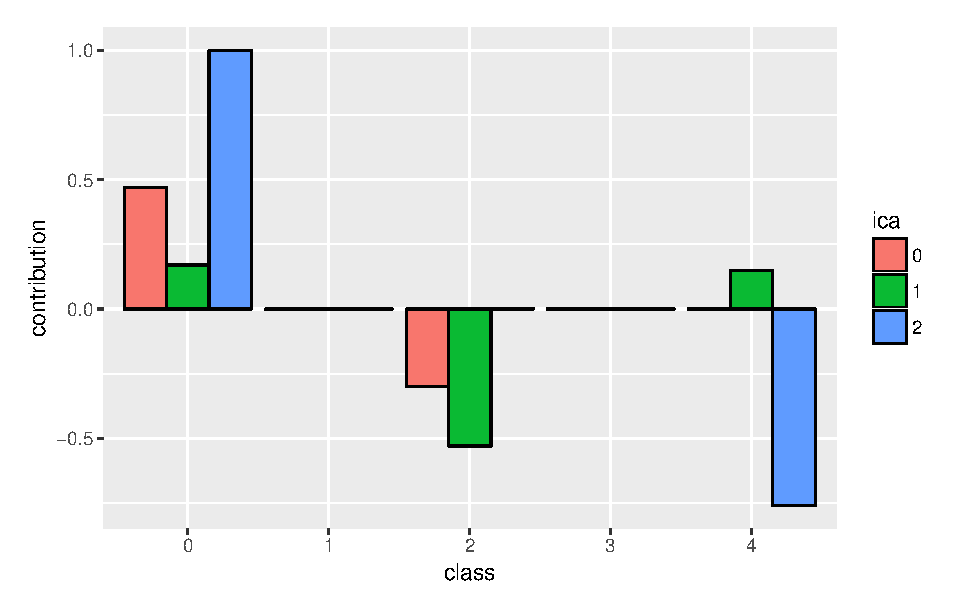
\includegraphics[width=0.65\textwidth]{./figures/ica_class_contribution.eps}
	\caption{Contribution of each ICA component in the classification final score}
	\label{fig:ica_contribution}
\end{figure}

Using the 64-dimensional feature-space vector of all the training set, we make a set of ICAs using different N values. With each one, we train a linear classifier to calculate the evaluation metric obtained over a validation set. We choose the minimal N that allows achieving maximum performance. The optimal N for this problem is $3$, achieving a $QWK_{val} = 0.790$ not far from the achieved by the original model without dimensionality reduction ($QWK_{val} = 0.800$).

Fig. \ref{fig:ica_contribution} shows the contribution of each component to the score of every class. We can see that the score markers are differentiating between class 0, 2 and 4.  Class 0 score contributions come from $ICA_0 > 0$, $ICA_1 > 0$ and $ICA_2 > 0$; being the class markers of the presence of disease $ICA_0 < 0$, $ICA_1 < 0$ and $ICA_2 < 0$. Analyzing the pixels with higher negative signals in the three components will give us the points that are contributing the most to the signaling of a possible presence of the disease. Backpropagating the scores of each one of this negative components will give a richer explanation with distinction between three possible independent causes of the final diagnostic given by the model.

A two-dimensional t-SNE visualization \cite{maaten2008visualizing} of the three components help us to enhance the visualization of the achieved class separation. In fig. \ref{fig:tsne} We can see how class 0, 2 and 4 classes are clearly separated. Class 0 and 1 are not properly separated and in the case of 3 and 4, although the separation is not perfect, it is possible to distinguish a different location of both classes in the graph.

\begin{figure}[h]
	\centering
	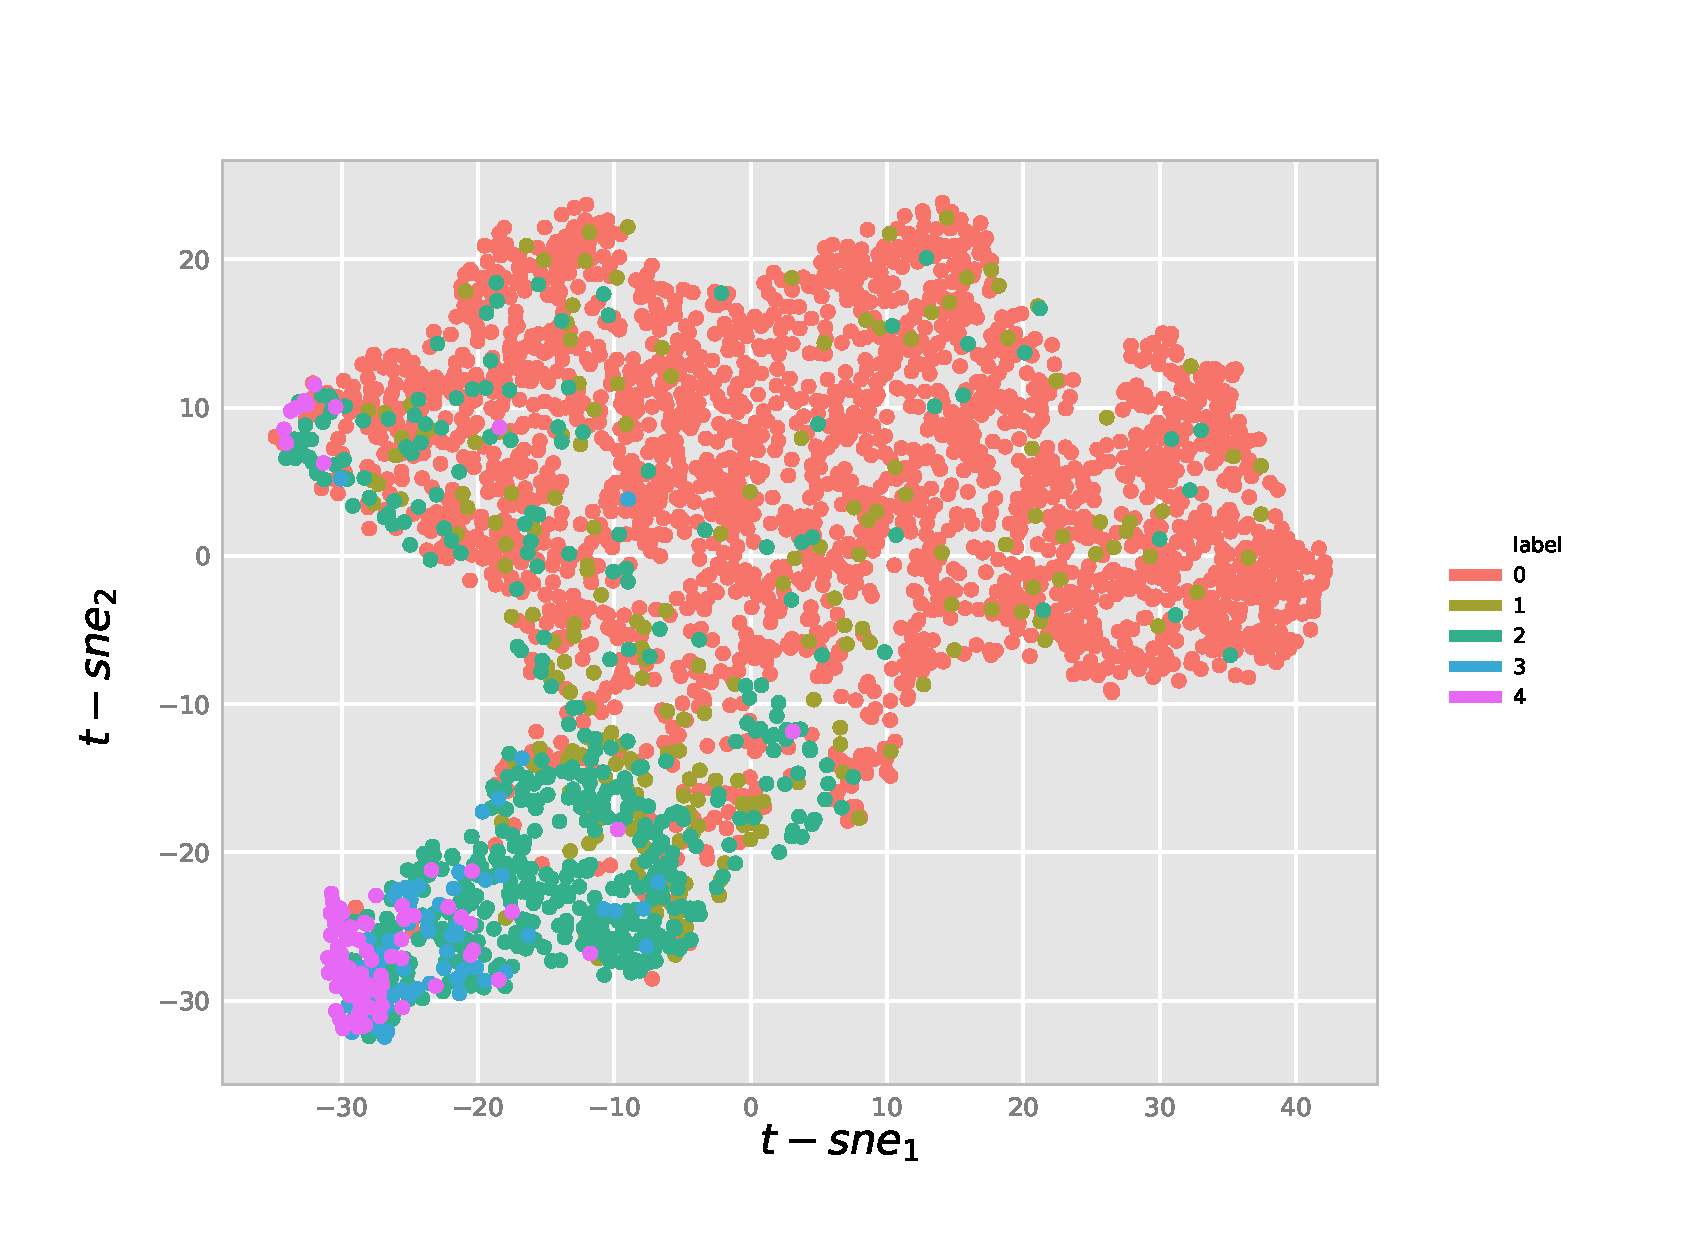
\includegraphics[width=0.65\textwidth]{./figures/tsne2d.eps}
	\caption{2D t-SNE visualization of validation set using three ICA components}  
	\label{fig:tsne} 
\end{figure}

\subsection{Score components contribution for a test sample}

We use a pixel-wise relevance propagation derived method for visualizing each ICA component independently. In this way it is possible to visualize the mathematically independent contributions enhancing the localization of different types of primary elements causing the disease. Figure \ref{fig:ica_components_hidden} shows two of the score maps that are calculated as intermediate steps. These maps are also useful when a general map of the lesion locations is enough.

\begin{figure}[h!]
	\centering
	\begin{subfigure}[b]{\textwidth}
		\centering
		\includegraphics[width=\textwidth]{./figures/c3/rf61.png}
		\caption{Hidden layer of receptive field 61x61}	
	\end{subfigure}
	\begin{subfigure}[b]{\textwidth}
		\centering
		\includegraphics[width=\textwidth]{./figures/c3/rf29.png}
		\caption{Hidden layer of receptive field 29x29}
	\end{subfigure}
	\hfill 
\caption{Visualization of hidden layer score maps for the three ICA components}  
	\label{fig:ica_components_hidden} 
\end{figure}

Figure \ref{fig:ica_components_c3} show the input space final scores. In this figure we show the points having contributions higher than a prestablished limit, in this case two standard deviations. This value is only informative and can be modified by the user.

\begin{figure}[h!]
	\centering
	\begin{subfigure}[b]{0.32\textwidth}
		\centering
		\includegraphics[width=\textwidth]{./figures/c3/retina_mICA0.png}
		\caption{$-ICA_0 > 2 \sigma_0$}	
	\end{subfigure}
	\hfill    
	\begin{subfigure}[b]{0.32\textwidth}
		\centering
		\includegraphics[width=\textwidth]{./figures/c3/retina_mICA1.png}
		\caption{$-ICA_1 > 2 \sigma_1$}
	\end{subfigure}
	\hfill 
	\begin{subfigure}[b]{0.32\textwidth}
		\centering
		\includegraphics[width=\textwidth]{./figures/c3/retina_mICA2.png}
		\caption{$-ICA_2 < 2 \sigma_2$}
	\end{subfigure}
	\caption{Visualization of a class 3 image. The original model scores are $C_0 = -661.0$, $C_1 = -294.1$,  $C_2 = -10.3$,   $C_3 = 70.3$,   $C_4 = 26.3$; $ICA_0 = 0.0174$, $ICA_1 = -0.0181$, $ICA_2 = -0.0237$}  
	\label{fig:ica_components_c3} 
\end{figure}

\section{Conclusions}\label{sec:conclusions}

In this paper we go a step further in the construction of a DL interpretable classifier design developing an algorithm able to differentiate between the independent causes involved in the classification decisions identifying, separating and visualizing them in the hidden and input space. For the Diabetic Retinopathy classification case, we identify only three independent elements that explain the severity of the DR disease. Our method allows not only the classification of retinographies but also the identification and localization in the image of the independent signs of the disease. The presented ICA score model is of general applicability and can be easily adapted for the usage in other image classification tasks.

%\section*{Acknowledgements}

%This work is supported by the URV grants 2017PFR-URV-B2-60, and the Spanish research project PI15/01150 (Instituto de Salud Carlos III) and Fondos FEDER. The authors would like to thank to Kaggle and EyePACS for providing the data used in this paper.

%\section*{References}
\bibliographystyle{unsrt}
\bibliography{retinopathy}

\end{document}